\subsection{Cross Sections as a function of the momentum imbalance along the neutrino direction} 
%Results in \tkipl }

Figure~\ref{figure:xsec_pl} gives the differential cross section as a function of \tkipl \ for interactions on the CH, C, H$_{2}$O, Fe, and Pb targets, respectively. 
\tkipl \ represents the longitudinal component of the momentum imbalance between the initial neutrino momentum and the sum of the final state lepton and hadron momenta.  This imbalance results from nuclear effects.  This variable and its extraction are discussed in a previous MINERvA paper~\cite{MINERvA:2018hba}. \tkipl\ can be calculated with the following equations,
\begin{equation}
    \tkipl = \frac{1}{2}R - \frac{m_{A'}^2 + \tkidelta^2}{2R}
    \label{eq:pl}
\end{equation}
\begin{equation}
    R \equiv m_{A} + p^\mu_L + p^p_L - E^\mu - E^p
\end{equation}
where $m_{A}$ and $m_{A'}$ are the masses of the atomic nucleus before and after interaction, and $p_L$ and $E$ are the momenta and energy of the muon and proton. Qualitatively, the MINERvA tune reproduces the data fairly well except for the case of interactions on Pb where the data exceeds the prediction. The uncertainties broken down by source for both the absolute cross sections and the cross section ratios as a function of \tkipl\ can be found in Fig.~\ref{fig:xsec_err_pl}. 


% tki_pl xsecs
\begin{figure}[h]  
	\centering
  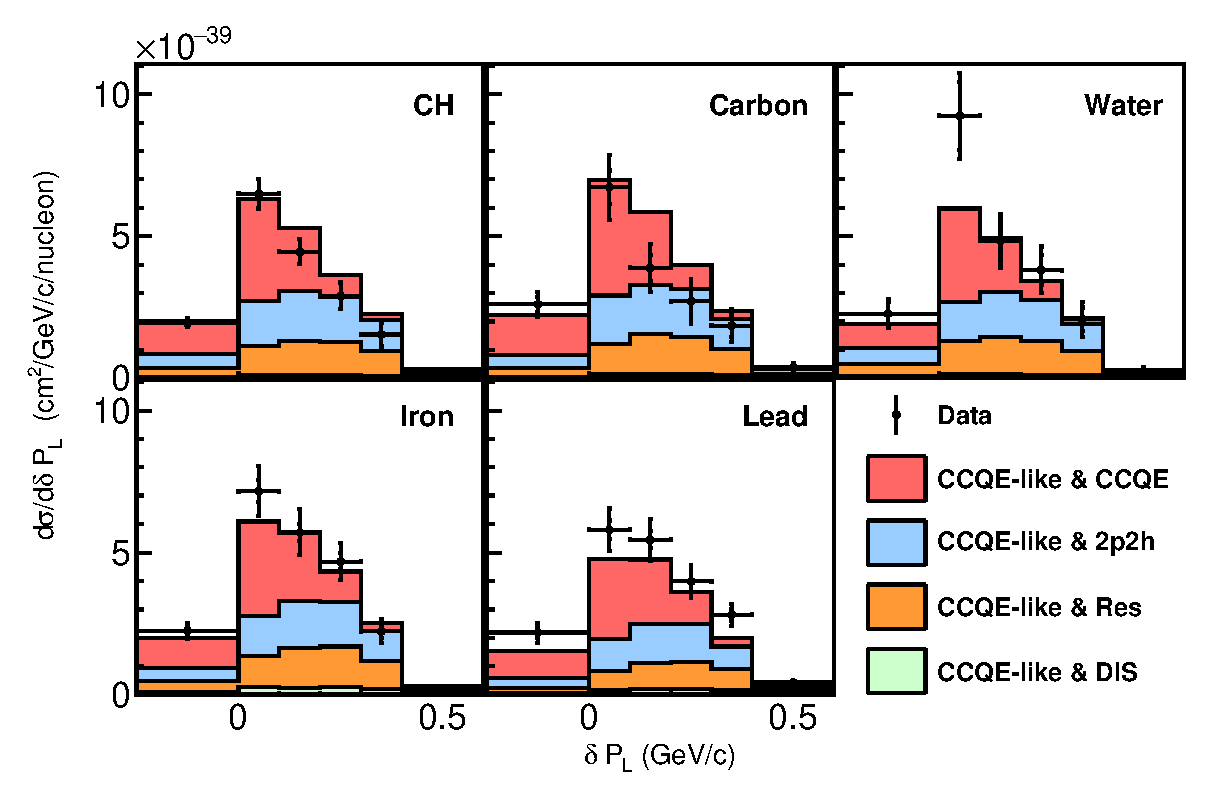
\includegraphics[width=\linewidth]{Figures/xsec_five_square/pl.eps}
	\caption{The differential cross section as a function of \tkipl\ for CH, C, H$_{2}$O, Fe, and Pb targets, along with the predictions for the different quasielastic-like signal processes.}
	\label{figure:xsec_pl}
\end{figure}


The results for a range of models are compared to the differential cross section as a function of \tkipl \ for the different targets in Fig.~\ref{fig:models_pl}.   Relative to the data,  NEUT has a larger cross section and the hN GENIE models and NEUT predict stronger nuclear effects than seen in the data for the larger targets.
The \chisq\ between the cross sections and the models can be found in Table~\ref{tab:pl}.

%show less evidence of nuclear effects than seen in the data while most of the other models show evidence of more nuclear effects than is seen in the data.  


% comparisons to generators p_l
\begin{figure}
    \centering
            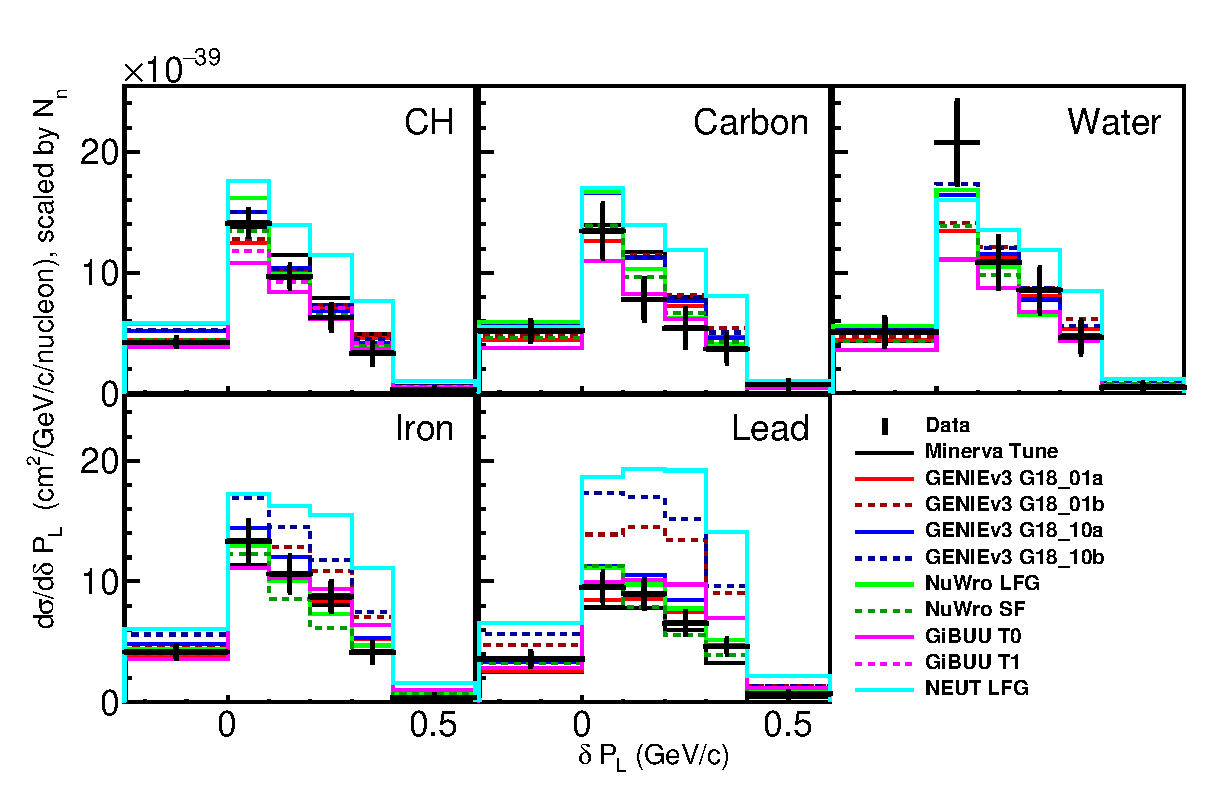
\includegraphics[width=\linewidth]{Figures/gencompare/pl_5square.eps}
    \caption{Cross section measurements and predictions as a function of \tkipl\ for different targets and for a selection of different generator and model choices. }
    \label{fig:models_pl}
\end{figure}

A plot of the ratio of the differential cross section as a function of  \tkipl \ for each nuclear target (C, H$_{2}$O, Fe, Pb) to that for scintillator is given in 
Fig.~\ref{Figure:Gencompare_pl_ratio}.  The data is fairly well described by the models for the smaller targets.  However,the model spread at high \tkipl \ for the Fe and Pb targets is large.
The \chisq\ between the cross section ratios and the models can be found in Table~\ref{tab:pl}.

\begin{figure}
    \centering
       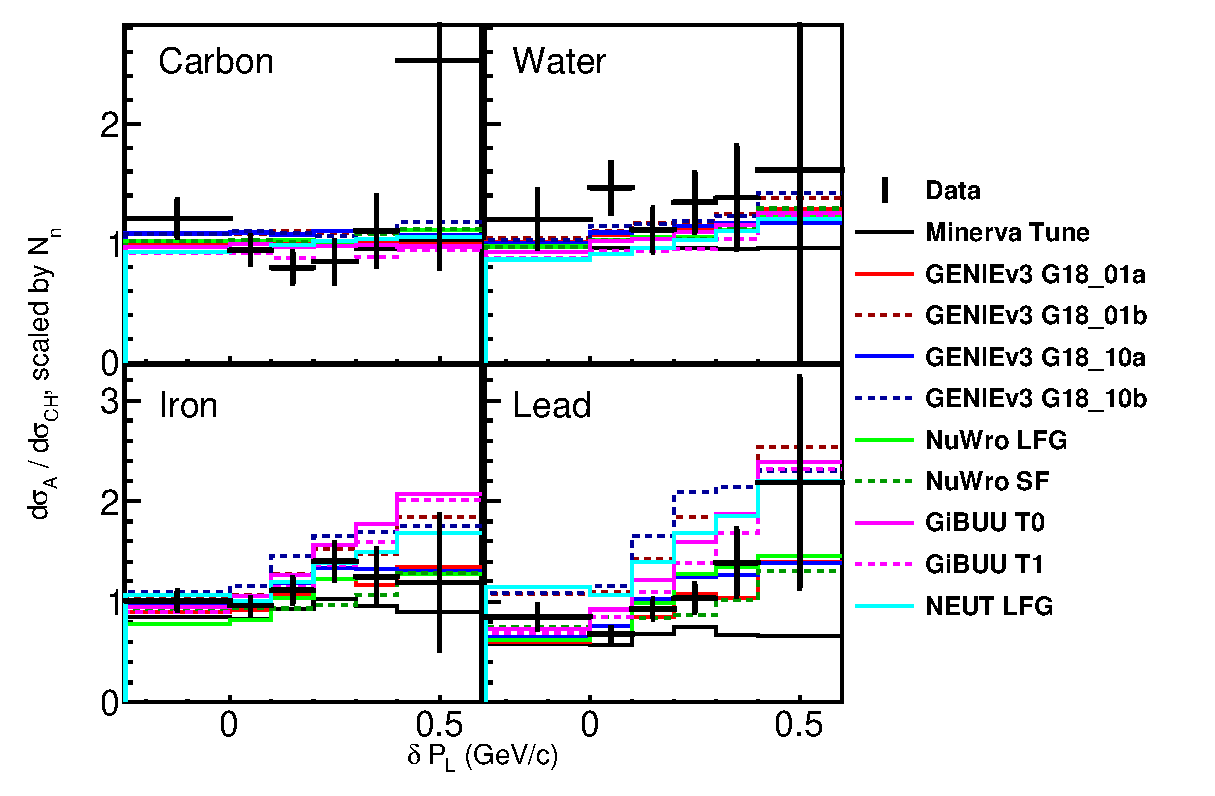
\includegraphics[width=\linewidth]{Figures/gencompare/pl_4square.eps}
    \caption{\tkipl\ cross-section ratio generator comparison for multiple targets.  Changes to the FSI model (GENIE ``a'' to ``b'') in GENIE change the cross section ratio throughout \tkipl\, and change the ratio more than changes to the 2p2h model (GiBUU T0 to GiBUU T1) or changes to the initial state (GENIE 1 to GENIE 10) or (NuWro LFG to NuWro SF).}
        \label{Figure:Gencompare_pl_ratio}
\end{figure}
